\documentclass{ctexbeamer}
\usetheme{beaver}


\setbeamertemplate{caption}[numbered]
\setbeamertemplate{blocks}[rounded][shadow=true]
% \graphicspath{{./figures}}

\usepackage[style=numeric]{biblatex}
\addbibresource{references.bib}
\renewcommand*{\bibfont}{\footnotesize}

\usepackage{minted}
\usepackage{listings}
\usepackage{xcolor}
\definecolor{codegreen}{rgb}{0,0.6,0}
\definecolor{codegray}{rgb}{0.5,0.5,0.5}
\definecolor{codepurple}{rgb}{0.58,0,0.82}
\definecolor{backcolour}{rgb}{0.95,0.95,0.92}
\lstdefinestyle{mystyle}{
   backgroundcolor=\color{backcolour},  
   commentstyle=\color{codegreen},
   keywordstyle=\color{magenta},
   numberstyle=\tiny\color{codegray},
   stringstyle=\color{codepurple},
   basicstyle=\ttfamily\footnotesize,
   breakatwhitespace=false,        
   breaklines=true,                
   captionpos=b,                  
   keepspaces=true,                
   numbers=left,                  
   numbersep=5pt,                
   showspaces=false,               
   showstringspaces=false,
   showtabs=false,                
   tabsize=4
}
\lstset{style=mystyle}

\usepackage{tikz}
\usetikzlibrary{overlay-beamer-styles}
 \tikzset{
    highlight on/.style={alt={#1{fill=red!80!black,color=red!80!black}{fill=gray!30!white,color=gray!30!white}}},
}

\usepackage{hyperref}
\hypersetup{
    colorlinks=true,
    % linkcolor=blue,
    urlcolor=red
}

\AtBeginSection[]{
  \begin{frame}
  \vfill
  \centering
  \begin{beamercolorbox}[sep=8pt,center,shadow=true,rounded=true]{title}
    \usebeamerfont{title}\insertsectionhead\par%
  \end{beamercolorbox}
  \vfill
  \end{frame}
}


\title{MPPT}
\subtitle{Modern Python Package Template}
\author{Mathew Shen}
% \date{\today}
% \date{August 2, 2023}
\date{2023 年 12 月 15 日}


% Define the colors for the beamer blocks
\usepackage{color}

\definecolor{myblack}{rgb}{0, 0, 0}

\setbeamercolor{block title}{bg=myblack,fg=white}
\setbeamercolor{block body}{bg=white,fg=black}


\begin{document}

\begin{frame}
\titlepage
\end{frame}

\begin{frame}
    \tableofcontents
\end{frame}



\section{Introduction}
\begin{frame}

    \begin{itemize}
        \item Package Management: Poetry
        \item Documentation: Mkdocs with Material theme
        \item Linters \& Formatter: Black, Isort, Flake8, Ruff, Mypy, Pre-commit, SonarLint
        \item Testing: Pytest, Hypothesis, Codecov
        \item Task runner: Makefile, Duty, Taskfile
        \item Miscellaneous: Changelog, License, Semantic Versioning, Contributing
    \end{itemize}

\end{frame}


\section{Package Management}

\begin{frame}{Most challenging problems}

    It's not a simple question...
    \footnote{The resources in the section are mostly from the book
    \textit{Software engineering at google: Lessons learned from programming over time}
    \cite{google-sre}}
    

    \begin{alertblock}{Most challenging problems in software engineering}
        Dependency management—the management of networks of libraries, packages, and dependencies 
        that we don't control—is one of the least understood and most challenging problems 
        in software engineering.
    \end{alertblock}

    \pause

    \begin{exampleblock}{A network of dependencies and their changes over time}
        The trick isn't just finding a way to manage one dependency—the trick is 
        how to manage a network of dependencies and their changes over time.
    \end{exampleblock}

\end{frame}

\begin{frame}{Conflicting Requirements and Diamond Dependencies}
    \begin{figure}
        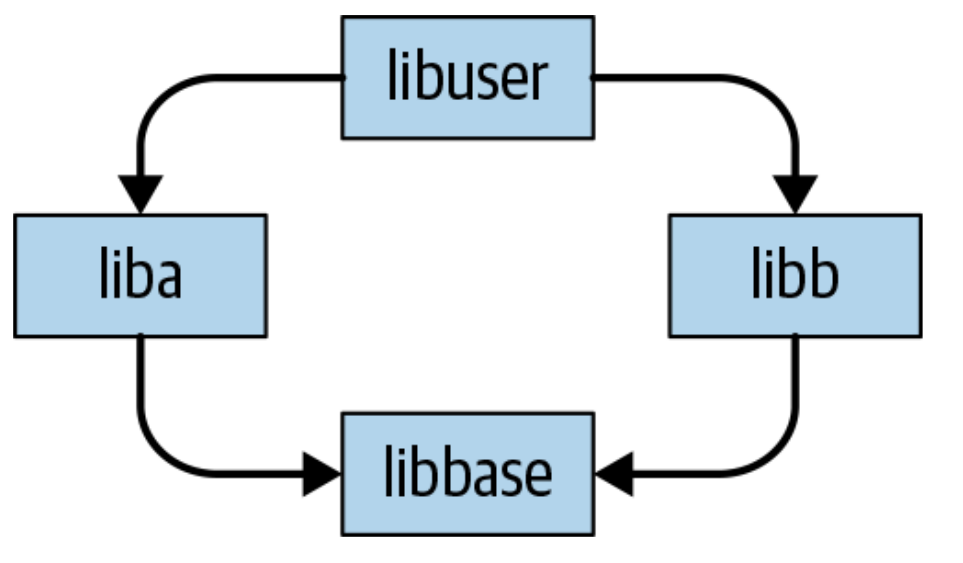
\includegraphics[width=0.3\textwidth, height=0.3\textheight]{./figures/diamond.png}
        \caption{Diamond Dependencies}
    \end{figure}

    \begin{alertblock}{Conflicting Requirements}
        If libbase ever introduces an incompatible change, 
        there is a chance that liba and libb , 
        as products of separate organizations, don't update simultaneously. 
        If liba depends on the new libbase version and libb depends 
        on the old version, there's no general way for libuser (aka your code) 
        to put everything together.
    \end{alertblock}

\end{frame}

\begin{frame}{Python's WELL KNOWN package management tool?}

    \begin{itemize}
        \item Java: Maven, Gradle
        \item Scala: SBT(Scala Build Tool), and Maven, Gradle
        \item JavaScript/TypeScript: NPM, PNMP
        \item Go: Go modules
        \item Rust: Cargo
        \item Python: Pip? Conda?
    \end{itemize}
\end{frame}


\begin{frame}{Python Environment}

    \begin{figure}
        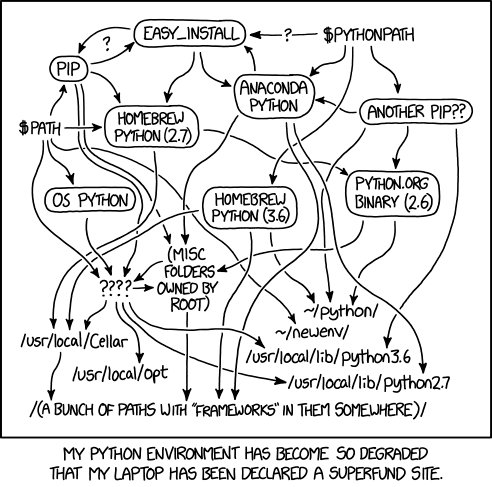
\includegraphics[width=0.6\textwidth, height=0.7\textheight]{./figures/python_environment.png}
        \caption{\href{https://xkcd.com/1987/}{XKCD: Python Environment}}
    \end{figure}

\end{frame}



\begin{frame}{Poetry}
    
    \begin{exampleblock}{Why Poetry?}
        \begin{itemize}
            \item More popular: Poetry(27.6K Star), Rye(7.6K Star), PDM(5.6K Star)
            \item Faster: \href{https://lincolnloop.github.io/python-package-manager-shootout/}{Python Package Manager Shootout}
        \end{itemize}
    \end{exampleblock}

\end{frame}


\begin{frame}{More details}
    See: \href{https://datahonor.com/mppt/package/}{https://datahonor.com/mppt/package/}
\end{frame}

\section{Documentation}
\begin{frame}{Mkdocs with Material theme}
    \begin{itemize}
        \item Markdown is easier/better(in a way) than reStructuredText(which is used by Sphinx)
        \item Material theme is Awesome!
    \end{itemize}
\end{frame}

\begin{frame}

    \begin{figure}
        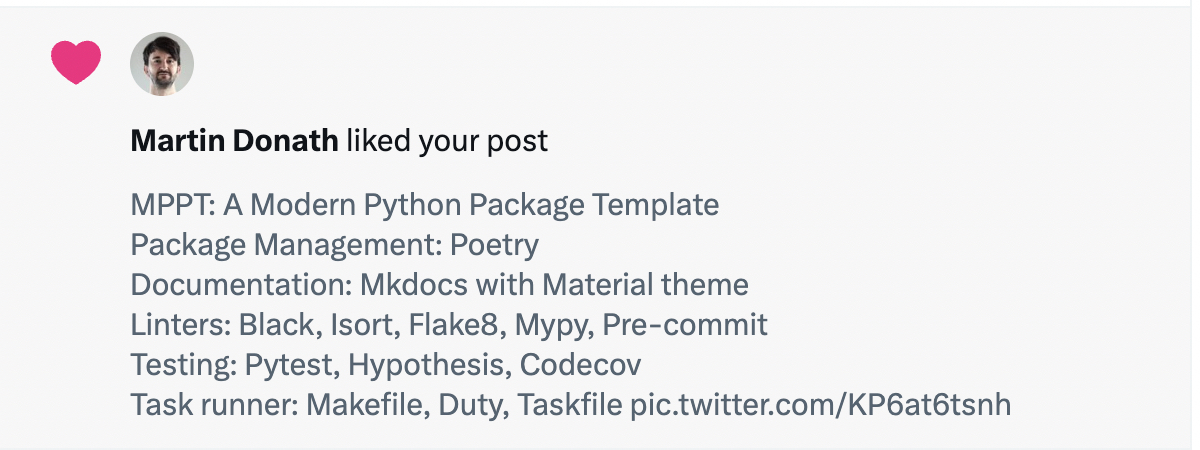
\includegraphics[width=0.99\textwidth, height=0.45\textheight]{./figures/like-martin.png}
        \caption{\href{https://twitter.com/MathewShen42/status/1731676210172756029}
        {Like from Martin Donath\footnote{Author of Material for MkDocs}}}
    \end{figure}


\end{frame}

\begin{frame}{More details}
    See: \href{https://datahonor.com/mppt/doc/}{https://datahonor.com/mppt/doc/}
\end{frame}


\section{Linter \& Formatter}

\begin{frame}[fragile]{Break code style is easy in Python}

How many code style mistakes in the code in \texttt{hello.py}?

\begin{lstlisting}[language=Python]
print ( "Hello, World" )
\end{lstlisting}

\pause

\begin{alertblock}{We got four code style mistakes in a one line hello world code.}
    \begin{itemize}
        \item \texttt{hello.py}:1:6: E211 whitespace before '('
        \item \texttt{hello.py}:1:8: E201 whitespace after '('
        \item \texttt{hello.py}:1:23: E202 whitespace before ')'
        \item \texttt{hello.py}:1:25: W292 no newline at end of file
    \end{itemize}
\end{alertblock}

\end{frame}

\begin{frame}{Linter \& Formatter}
    \begin{exampleblock}{Solution1: Black, Isort, Flake8, MyPy}
        \begin{itemize}
            \item Black: Code Formatter
            \item Isort: Style Linter for Import Statements
            \item Flake8: Error \& Style Linter \& Complexity Analysis
            \item MyPy: Type Checker
        \end{itemize}
    \end{exampleblock}

    \pause

    \begin{exampleblock}{Solution2: Black, Ruff, MyPy}
        Ruff: Linter \& Formatter
    \end{exampleblock}

    \pause 

    \begin{exampleblock}{Pre-commit}
        We can use pre-commit to manage all the liners and formatters together.
    \end{exampleblock}

\end{frame}

\begin{frame}{More details}
    See: \href{https://datahonor.com/mppt/linter/}{https://datahonor.com/mppt/linter/}
\end{frame}

\section{Testing}
\begin{frame}{Testing}
    \begin{itemize}
        \item Pytest
        \item Hypothesis
        \item Codecov
    \end{itemize}
\end{frame}

\begin{frame}[fragile]{Hypothesis for property-based testing}

Property-based testing is popularised by the Haskell library Quickcheck.
\footnote{\tiny \href{https://hypothesis.readthedocs.io/en/latest/index.html}{Hypothesis doc}}

\begin{lstlisting}[language=Python]
from hypothesis import given
from hypothesis.strategies import text


@given(text())
def test_decode_inverts_encode(s):
    assert decode(encode(s)) == s

\end{lstlisting}

\end{frame}

\begin{frame}{More details}
    See: \href{https://datahonor.com/mppt/test/}{https://datahonor.com/mppt/test/}
\end{frame}

\section{Task runner}
\begin{frame}{Task runner}
    \begin{itemize}
        \item Makefile
        \item Taskfile
        \item Duty
        \item Typer
    \end{itemize}
\end{frame}

\begin{frame}{More details}
    See: \href{https://datahonor.com/mppt/task/}{https://datahonor.com/mppt/task/}
\end{frame}

\section{Miscellaneous}
\begin{frame}{Miscellaneous}
    \begin{itemize}
        \item \href{https://keepachangelog.com/en/1.1.0/}{Keep a Changelog}
        \item \href{https://semver.org/}{Semantic Versioning}
        \item \href{https://choosealicense.com/}{Choose an open source license}
        \item \href{https://shields.io/}{Badge: Shield.io}
        \item \href{https://guides.github.com/activities/contributing-to-open-source/}{Contributing to Open Source on GitHub}
    \end{itemize}
\end{frame}

\begin{frame}{More details}
    See: \href{https://datahonor.com/mppt/miscellaneous/}{https://datahonor.com/mppt/miscellaneous/}
\end{frame}

\begin{frame}{References}
    \printbibliography
\end{frame}


\section{QA}


\end{document}

